
\def \R2{\mathbb{R}^2}
\def \R3{\mathbb{R}^3}
\def \Rn{\mathbb{R}^n}

\def \itW{\mathit{W}}

\def \itK{\mathit{K}}
\def \bfp{\mathbf{p}}

\chapter{基于BA的单目相机实时重建的经典算法(PTAM)介绍}

本章节将重点讨论并实现基于BA的单目相机实时重建经典算法:PTAM。该算法是基于关键帧特征和BA的稀疏重建算法的开山鼻祖,具有重要的意义。

\section{PTAM算法的介绍}
首先我们将简述PTAM\cite{Klein2007}(Parallel Tracking and Mapping)实现单目相机SLAM的原理。单目相机模型(Monocular SLAM)不同于多目相机模型,实时追踪时相机视界中的点不能和其它相机视界中的点进行匹配或者实现三角定位,只能和自己的关键帧匹配,从而加大了3D重建中定位(即深度信息求解)的难度。一般的PTAM算法首次提出利用双线程,将全局BA和相机姿态估计这两个任务分离,从而大幅提高了计算效率,使得单目相机实时追踪特征点,实现三维重建成为可能。

PTAM算法主要思想是将Tracking和Mapping两个过程放在不同的管线(进程)中进行: Tracking 进程专门实现相机位置的估计,Mapping 进程则用于进行关键帧之间的误差消除。

\section{PTAM算法工作的基本流程}
如果记$\itW$为真实世界的坐标系,PTAM算法将维护一个关键帧集合: $Img=\{I_1,I_2,\ldots,I_m\}$,这\(m\)个关键帧分别对应\(m\)个相机坐标系 $\itK_i$,以及一个三维重建的结果。我们用 $E_{\itK_i\itW}$ 表示从世界坐标系到相机坐标系的仿射变换(Affine Transformation)。


\subsection{PTAM管线之一: Tracking}


追踪进程需要解决如下的问题:

当读入了新的关键帧之后,原来算法在重建过程中提取的3维空间中的特征点现在在照片中的坐标是什么?现在的相机姿态应该怎么估计? 

我们假定程序可以从映射进程得到一个关键帧集合 $Img$ 以及3维重建的特征点的坐标集合(相对于世界坐标系)$P=P_\itW=\{\bfp_{1\itW},\ldots,\bfp_{s\itW}\}$,为了统一形式,将第$j$个点坐标记为 $\bfp_{j\itW}= (p_{jx},p_{jy},p_{jz},1)$。

根据已知结论,仿射坐标系变换对应公式为

\begin{equation}
\bfp_{jK_{t+1}}= E_{K_{t+1}\itW} \bfp_{j\itW}
\end{equation}

为了把三维空间中的视界投影到二维空间,算法遵循\cite{Klein2007}中的FOV相机模型,构建一个$\mathbb{R}^3$到 $\mathbb{R}^2$ 的映射为:

\begin{equation}
\label{eq:FOV}
f(x,y,z,1)=(u_0,v_0) + (x/z,y/z) 
\begin{bmatrix}
       f_u  & 0 \\
       0 & f_v  \\
\end{bmatrix} \frac{r'}{r}
\end{equation}
\begin{equation}
r= \sqrt{\frac{x^2+y^2}{z^2}}
\end{equation}

\begin{equation}
r'= \frac{1}{\omega} arctan(2rtan\frac{\omega}{2})
\end{equation}

其中我们假定焦距$f_u,f_v$,主点位置$(u_0,v_0)$和畸变系数$\omega$已知。这时对于实时相机姿态的更新,相当于对于 \autoref{eq:FOV} 求微分,在假定线性运动的情况下更新相机姿态的变换仿射矩阵。若我们设从上一关键帧到下一个关键帧的仿射变换矩阵为$T$,则有以下的关系成立:

\begin{equation}
E_{K_{t+1}\itW}  = T E_{K_{t}\itW} = exp(\mu) E_{K_{t}\itW}
\end{equation}

其中$\mu$为6维向量,代表矩阵 $T$的6个自由度。所以问题转化为: 根据图像中特征点$(u,v)$的变化和在每个特征点三维空间中的预估位置,求解$\mu,T$的取值。


我们假定点$p$为我们需要定位的特征点,则我们首先需要在当前的关键帧图像中找到该点的新投影坐标$(\hat{u},\hat{v})$。为此,我们构造图像的尺度空间,利用 %\citep{}
的FAST-10\cite{Rosten2006}计算角点的方法提取可能的特征点。在假定相机移动很慢的情况下,特征点匹配算法从上一帧的位置开始,在一定的半径阈值内,在对应的视界空间上,依据设计好的评价函数(scoring function)进行搜索。
算法会在搜索过程中得到一个坐标$(\hat{u},\hat{v})$,以及 $\sigma=2^l$ 作为视界空间金字塔中搜索对应的层数。

\begin{figure}[!htbp]
\centering
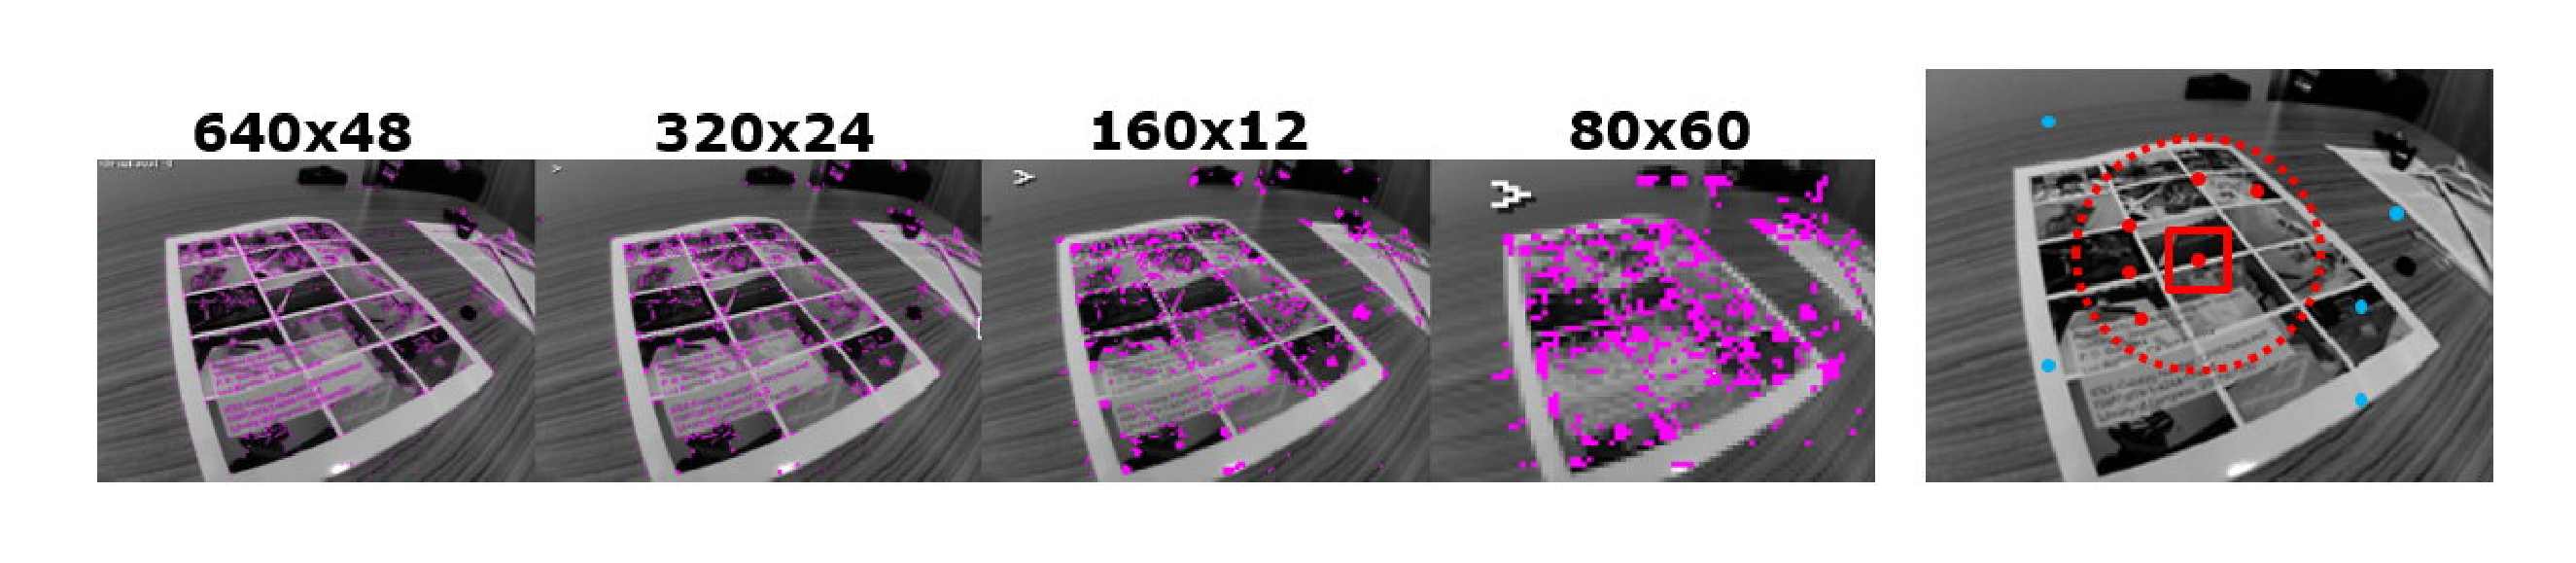
\includegraphics[width=14cm]{PTAM01.pdf}
\caption{视界空间中利用FAST提取特征点和搜索对应特征点示意图,左图表示视界空间的down sampling,以及基于FAST方法的特征点选取,右图为在对应的尺度空间中搜索对应的特征点}
\label{fig:PTAM01}
\end{figure}
在得到所有特征点的信息之后,算法求解以下的优化问题
计算相机姿态的更新(设$P_{t+1}$为当前特征点集合):

\begin{equation}
\label{eq:post_update}
\underset{\mu}{argmin} \sum_{j\in P_{t+1}} \psi( \frac{\lVert\mathbf{e}_j\rVert}{\sigma_j} , \sigma_T)
\end{equation}
\begin{equation}
\mathbf{e}_j= (\hat{u_j},\hat{v_j})- f(exp(\mu)E_{K_{t}\itW} \mathbf{p_j})
\end{equation}

这里 $\psi$ 为 Tukey loss\cite{A86robuststatistics}:

\begin{equation}
\psi(x,c)= 
\begin{cases}
x(1-\frac{x^2}{c^2}) & \text{for }|x|<c \\
0  &  \text{for }|x|>c
\end{cases}
\end{equation}

为了保证算法的稳定性,追踪进程会进行两次:第一次会从三维模型中抽取50个特征点投影匹配,第二次则抽取1000个特征点进行匹配。同时,如果在特征点投影搜索配对的过程中,如果特征点搜索失败的比率大于某一个阈值的话,算法将会判定这一帧失效,并且自动舍弃(这可能是由于抖动,位移量过大特征点不在视界中等多种原因造成)。


\subsection{PTAM管线之二: Mapping}

在追踪进程持续运行的同时,映射进程会根据追踪进程估计的相机姿态,完成关键帧的选取及三维重建的主要任务。为此,算法首先在初始化阶段,需要用户指定视频流中的两帧(第一帧一般为起始帧),单独进行第一次特征点配对。这样做的目的有两个,一方面是为了利用五点法求解相机模型中的固有参数,另一方面是为了先定位特征点到三维空间中作为初始信息。

\subsubsection{关键帧的选择和插入}
在程序进程中,当视频流被读入之后,对于每一帧图像,算法需要判断是否需要把该帧图像加入关键帧集合。判断主要依据是距离上一关键帧的时间和预估的相机距离,以及图像的质量。在选定关键帧之后,根据追踪进程返回的信息,结合上一关键帧的对应特征点信息,定位深度,从而把特征点加入到三维重建模型中。

\subsubsection{利用BA(Bundle Adjustment)校正}
为了消除帧与帧之间的积累误差,映射进程还需要对整体的投影误差和进行一个优化,即所谓的BA。算法对于所有关键帧求解一次优化问题,也会对局部的几个特征点求解局部的优化问题,它们有以下形式:

\begin{equation}
\underset{\{\mu\},\{\mathbf{p}\}}{argmin} = \sum_{i=1}^{N} \sum_{j\in P_i} \psi(\frac{\lVert\mathbf{e}_j\rVert}{\sigma_j},\sigma_T)
\end{equation}

这里的计算将会采用Levenberg-Marquardt BA算法(详见\cite{Hartley2004})。在完成校正之后,新的特征点的三维信息和关键帧信息将作为追踪进程的输入,传入Tracking进程,两个进程在工作的时候将会保持相互的通信,这样最大程度上保证算法运行的流畅度。上述算法的核心过程,在下方\autoref{fig:PTAM_process}中进行了简要的总结。

\newpage
% 流程图定义基本形状
\tikzstyle{startstop} = [rectangle, rounded corners, minimum width=3cm, minimum height=1cm,text centered, draw=black ] %, fill=red!30]
\tikzstyle{io} = [trapezium, trapezium left angle=70, trapezium right angle=110, minimum width=3cm, minimum height=1cm, text centered, draw=black ]%,fill=blue!30]
\tikzstyle{process} = [rectangle, text width=3cm ,minimum width=3cm, minimum height=1cm, text centered, draw=black]%,fill=orange!30]
\tikzstyle{smallprocess} = [rectangle, text width=2cm ,minimum width=2cm, minimum height=1cm, text centered, draw=black]%,fill=orange!30]
\tikzstyle{decision} = [diamond, aspect=2.5, minimum width=1cm, minimum height=1cm, text centered, draw=black]%,fill=green!30]
\tikzstyle{arrow} = [thick,->,>=stealth]

\begin{figure}
\centering
\begin{tikzpicture}[node distance=2cm]

%定义流程图具体形状
\node (Tstart) [startstop] {Tracking};
\node (in1) [process, below of=Tstart] {接收Mapping进程的信息};
\node (pro1) [process, below of=in1] {提取当前帧特征点};
\node (pro2) [process, below of=pro1] {投影匹配特征点};
\node (pro3) [process, below of=pro2] {根据\autoref{eq:post_update}求解相机姿态变化};
%\node (out1) [io, below of=pro2a] {Output};
%\node (stop) [startstop, below of=out1] {Stop};



\node (Mstart) [startstop, right of= Tstart, xshift=7cm] {Mapping};
\node (stereo) [process, above of = Mstart] {初始化};
\node (Mpro1)  [process, below of = Mstart] {关键帧判定与添加};
\node (Mdec1)  [decision, below of = Mpro1, yshift=-0.6cm] {是否全局收敛};
\node (Mpro2)  [smallprocess, left of = Mdec1, xshift=-2cm] {全局BA};
\node (Mdec2)  [decision, below of = Mdec1, yshift=-0.8cm] {是否局部收敛};
\node (Mpro3)  [smallprocess,left of =Mdec2, xshift=-2cm] {局部BA};
\node (Mpro4)  [process, below of =Mdec2] {更新关键帧和深度信息};
%连接具体形状
\draw [arrow](Tstart) -- (in1);
\draw [arrow](in1) -- (pro1);
\draw [arrow](pro1) -- (pro2);
%\draw [arrow](dec1) -- (pro2a);
%\draw [arrow](dec1) -- (pro2b);
%\draw [arrow](dec1) -- node[anchor=east] {yes} (pro2a);
%\draw [arrow](dec1) -- node[anchor=south] {no} (pro2b);
\draw [arrow](pro2) -- (pro3);
%\draw [arrow](pro2a) -- (out1);
%\draw [arrow](out1) -- (stop);
\draw [arrow](pro3) |- +(-2.5,-1) |- (in1);
\draw [arrow](stereo) -- (Mstart);
\draw [arrow](Mstart) -- (Mpro1);
\draw [arrow](Mpro1) -- (Mdec1);

\draw [arrow](Mdec1) -- node[anchor=south] {否} (Mpro2);
\draw [arrow](Mdec1) -- node[anchor=west] {是} (Mdec2);
\draw [arrow](Mdec2) -- node[anchor=west] {是} (Mpro4);
\draw [arrow](Mdec2) -- node[anchor=south] {否} (Mpro3);

\draw [arrow](Mpro2) |- +(0,-1.3) -- +(4,-1.3) -- (Mdec2);
\draw [arrow](Mpro3) |- (Mpro4);

\draw [arrow](Mpro4) -| +(2.5,1) |- (Mpro1);

\draw [arrow](in1) -- node[anchor=north] {匹配特征点对,相机姿态估计} (Mpro1);
\draw [arrow](Mpro1) -- node[anchor=south] {关键帧信息,三维重建模型} (in1);

\end{tikzpicture}

\caption{基于BA的单目经典算法PTAM的流程示意图}
\label{fig:PTAM_process}

\end{figure}


\section{PTAM算法的实际效果}

本节重点比较和讨论对于PTAM算法运行效果。

\subsection{在一般电脑上运行}

我们实现了PTAM在Win10 32bit, openCV 3.2, VS2015的实际环境下,利用笔记本摄像头或者与手机摄像头相连的方式,在一般的笔记本电脑上运行的成果,运行的实际效果如下图所示。对于开放的场景(如寝室内部),实际测试中十分卡顿,掉帧严重,且追踪能力不强。对于特定的平面场景(如桌面),实际测试结果(例如\autoref{fig:PTAMrun})也不近如人意,虽然有时会正确侦测到平面并完成渲染,但有时三维重建和平面的探测结果非常奇怪,十分不鲁棒。。且初始化的stereo init非常依赖初值,可能需要$1\sim5$秒的时间

\begin{figure}[!htbp]
\centering 
\subfloat[实际场景追踪]{
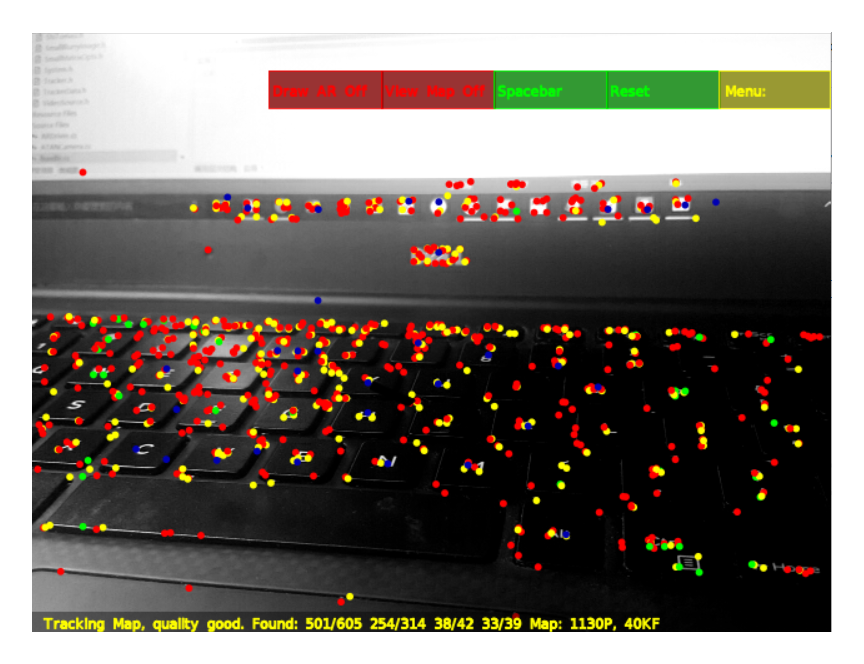
\includegraphics[width=4.5cm]{PTAMrun01.png}}
\subfloat[平面探测与AR渲染]{
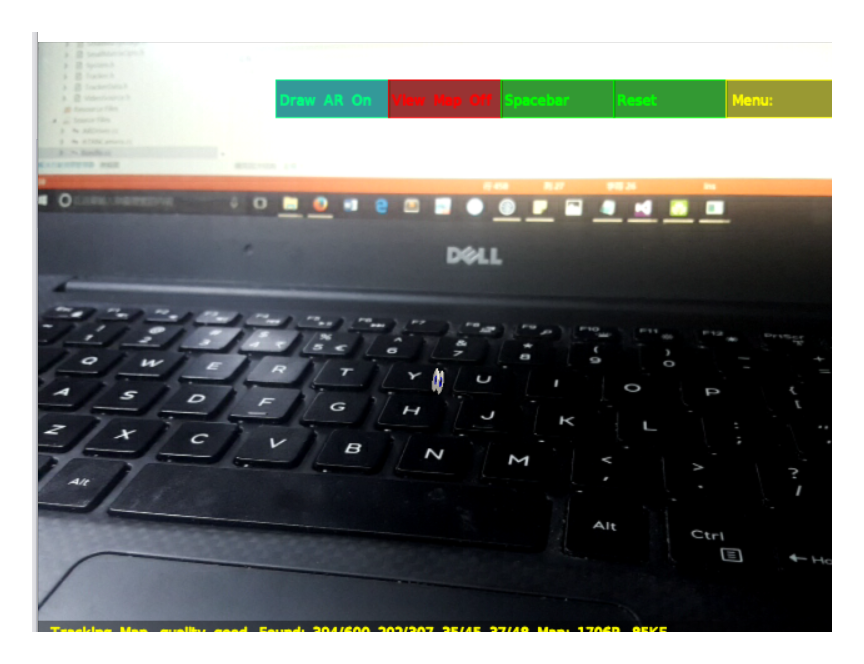
\includegraphics[width=4.5cm]{PTAMrun02.png}}
\subfloat[稀疏三维地图重建]{
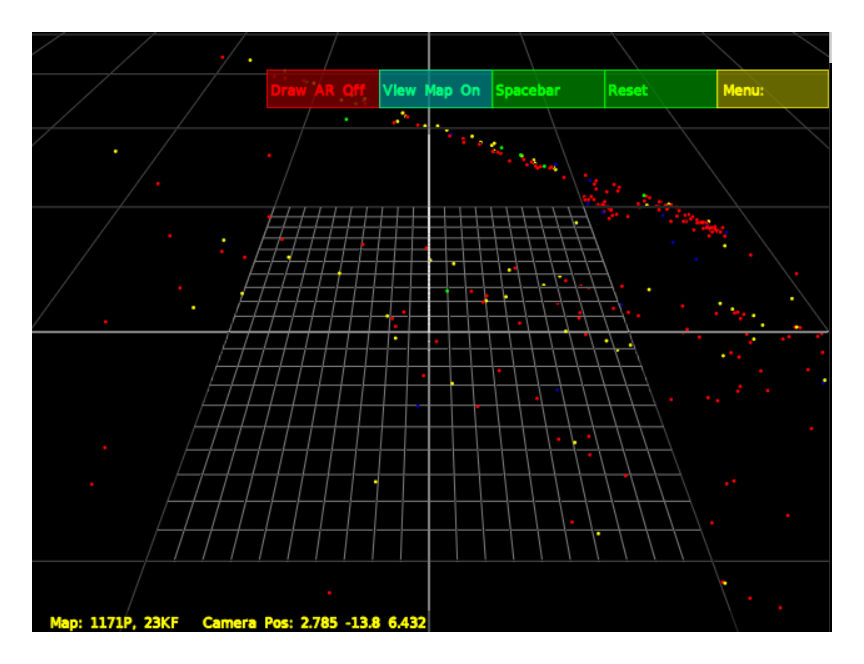
\includegraphics[width=4.5cm]{PTAMrun03.png}}
\caption{PTAM在电脑上实际运行的效果}
\label{fig:PTAMrun}
\end{figure}

\subsection{在智能手机上运行}

智能手机的性能会是制约此类算法在手机上表现的一个重要因素,\cite{Klein2009}中尝试把PTAM的系统移植到Iphone中,得到了\autoref{fig:PTAMcell01}所示的结果。我们虽然并未实现该算法,但可以预见该算法在手机上的运算效率并不会很高。

\begin{figure}[!htbp]
\centering
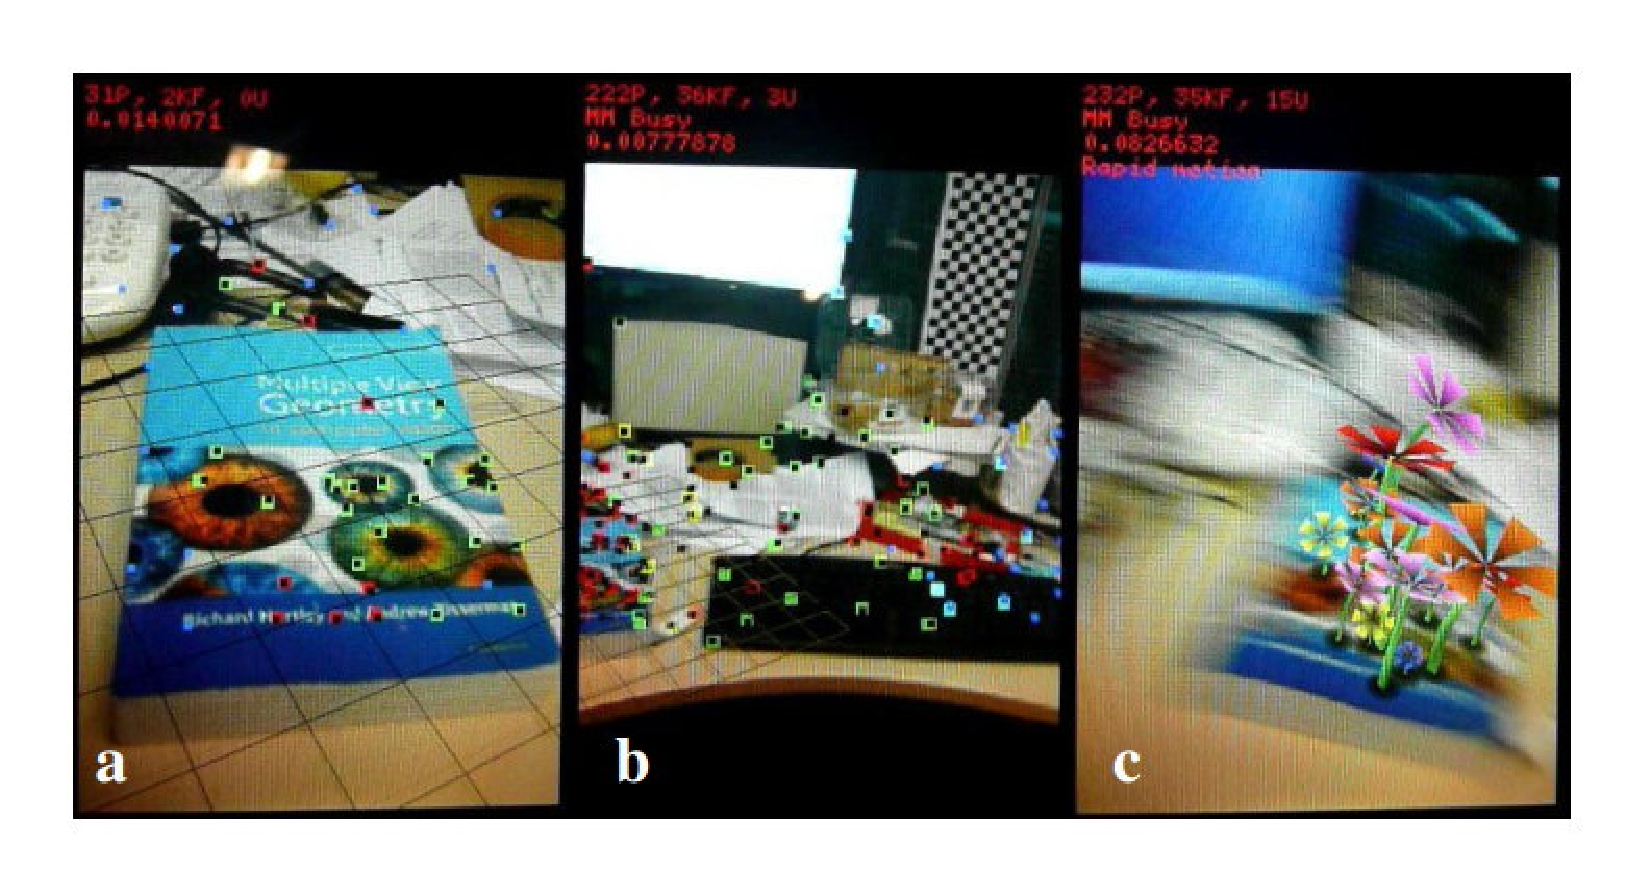
\includegraphics[width=12cm]{PTAMcell01.pdf}
\caption{在智能手机上运行的结果,(a)图为起始状态,(b)图表现了特征点的追踪,(c)图表示了在运动过程中的平面捕捉与AR渲染。由于手机运算能力限制,特征点数量较PC端大幅减少}
\label{fig:PTAMcell01}
\end{figure}
